\documentclass[a4paper,10pt,titlepage,twocolumn]{article}
    \usepackage[left=1in,right=1in,top=1in,bottom=1in]{geometry}
    \usepackage{graphicx}
    \usepackage{url}
    \usepackage{listings}
    \usepackage{xcolor}

    \definecolor{background}{HTML}{EEEEEE}
    
    \lstdefinelanguage{json}{
    basicstyle=\normalfont\ttfamily,
    numbers=none,
    numberstyle=\scriptsize,
    stepnumber=1,
    numbersep=10pt,
    showstringspaces=false,
    breaklines=true,
    frame=,
    backgroundcolor=\color{background},
    literate=,
}

\begin{document}
\linespread{1.5}
    \title{COMP90015 Distributed Systems \\Project 2 \\Security and UDP\\}
    \author{\\\Large \textit{Team Koala} \\
    \\
        \begin{tabular}{|c|c|c|}
        \hline
        Members &loginName&Emails \\ \hline
        Yue Guo & guoy7 &\url{guoy7@student.unimelb.edu.au}  \\ 
        Runze Nie & runzen & \url{runzen@student.unimelb.edu.au} \\
        Cheng Qian & cqq & \url{cqq@student.unimelb.edu.au} \\ 
        Junyi Wu & junyiw7 & \url{junyiw7@student.unimelb.edu.au} \\ \hline
    \end{tabular}}
    \date{}
    \maketitle
    \section{Introduction}
    Based on the Bitbox system in Project 1, this project focuses on two primary sections -- Security and UDP connection. This report is going to discuss the implementation and some relevant questions in this project.
    \section{Security}
    \subsection{Implementation}
    Asymmetric cryptography, usually called public key cryptography, uses the public key to encrypt the message and the encrypted message can only be decrypted by the owner of the private key. Asymmetric cryptography provides stronger protection to sensitive information because even if the server leaks the public key, the attacker will not be able to decrypt the message as long as the private key is safe. Asymmetric cryptography is commonly used in the initialization stage of a connection. Then the connection will be switched to symmetric cryptography because it is much more efficient.
\\When building a file permission scheme in BitBox, identity authentication can be quite important, and the asymmetric cryptography is suitable for authentication procedures. The client should generate the key pair and share the public key with the server when the identity of the client is registered at the server end. Every time the user wants to start a connection, the client end sends an authentication request to the server, and the server will find the public key of the user and use it to encrypt a random number. If the client can use the corresponding private key to decrypt the message and send it back to the server, the server will give permission to the client and switch to the symmetric cryptography after exchanging the symmetric key for the session. 
\\The detailed permission of a user is specified by a configuration file saved at the server end, which specifies whether a user or group can read, write or execute a specific file or directory. Every time a file or directory manipulation request is received by the server end, the server will check the authorization of the user in the permission table, and decide whether to provide the permission or not.
\\To implement the scheme mentioned above, the server administrator should make sure the public keys and usernames are mapped correctly and the permission of different users and groups are configured properly. Moreover, the administrator should also consider both the group and individual permission of a user, for example, a user may be a member of multiple groups. When confirming the client has the private key, we should also use other techniques to keep the procedure of sending the random number safe, such as hashing.
    \subsection{Grant Permission}
    As the public/private keys are generated in pairs, the user can access the files by verifying the Authentication key. The peer owned the private key, which pairs the public key holding by the server will have access to the file system. This can be considered as the user own this part of files or directories due to the reason that others without the private key can not access them. As the server, it can also grant authority to users like command $chown$ works in Linux. It can allow administration in different levels to different users, including view-only or read/write.
    \subsection{Limitations}
    It seems no severe limitations in this kind of approach as following reasons.
    \begin{itemize}
        \item This approach is like SSH connection, which has been widely used in the real world. 
        \item For the permission of users, it can be implemented like $chown$ command in Linux. It can grant permission to users by different levels, like read-only or read and write.
    \end{itemize}
    \subsection{Protocol}
    It is feasible to make changes on the current system so that the clients are enabled to access the files in the peers. However, with the current protocol, any file in the share directory of Bitbox is available for any client, and so do the basic file operations on these files namely reading, modifying, and deleting. Therefore, to achieve the file permission scheme described above, the current protocol implemented for Bitbox should be modified.
    \\First of all, each peer could maintain a file (text or CSV) containing the information of all files and directories inside the share directory. It should be maintained outside the $share$ directory as the configuration file of Bitbox peers in this project. The content of this file and several examples given are shown in the table below. It contains not only the pathnames of the files and directories in the $share$ directory, but also the information concerned with who is the author (shown as Account Name), which group of users is allowed to read or write the corresponding file and directory. For instance, the Table \ref{table_1} indicates that the directory ‘share/client\_1’ is created and owned by client\_1, and only he/she can create or modify files or directories in this directory, while client\_2 and clien\_3 are only allowed to view the content of the files or directories.

    \begin{table}[h]
        \begin{center}
            \begin{tabular}{|p{1.15cm}|p{1.15cm}|p{1.15cm}|p{1.15cm}|p{1.15cm}|}
                \hline
                Path- name & Type & Account & Write & Read \\ \hline
                share/ client\_1&$direct- ory$&client\_1&client\_1 &client\_1 client\_2 client\_3 \\ \hline
                share/ client\_1/ dog.jpg & $file$&client\_1&client\_1 client\_2 &client\_1 client\_2 client\_3 \\ \hline 
                share/ client\_2& $direct- ory$ &client\_2&client\_2&client\_2 \\ \hline
                share/ client\_2/ cat.jpg & $file$ &client\_2&client\_2&client\_2 \\ \hline
            \end{tabular}
            \caption{File Information}\label{table_1}
        \end{center}
    \end{table}
    
To make use of the table above, the protocol should be capable with the following features. In terms of the reading permission, when the client sends the command to the peer requiring to view the content of a file or a directory, despite the target pathname, the command message should also contain the account information of the client, two example messages are shown below. 
    
    \begin{lstlisting}[language=json,firstnumber=1,title=Message 1]
{
    "command":"READ_FILE_REQUEST",
    "pathname":"client_1/dog.jpg",
    "account":"client_1"
}
    \end{lstlisting}
    \begin{lstlisting}[language=json,firstnumber=1,title=Message 2]
{
    "command":"READ_FILE_REQUEST",
    "pathname":"client_2/cat.jpg",
    "account":"client_1"
}
    \end{lstlisting}
    Then the peer received this message should check if this account is allowed to access the target pathname, by retrieving the table above, and decided whether to display the target file or directory to the client side. For the two example messages above, the first one can be permitted according to the table1, while the second one will be rejected as the pathname ‘client\_2/cat.jpg’ can only be accessed by client\_2. It is similar for the writing permission, the only difference is that the peer received the writing request message should decide whether to commit the changes made by the client to the $share$ directory.
    \\The overall interaction diagram is shown in Figure \ref{figure} below. Each peer in this distributed system maintains the same files and directories, and one of UDP and TCP can be utilized to ensure the concurrency between these nodes. As for the clients, they are able to connect to one of these peers via public/private key technology using TCP, and send command to the peer to get its connection information, control its connections such as connecting to or disconnecting from a specific peer, as well as read or write files and directories in the share directory, according to the file information table described above.
    \begin{figure}[h]
        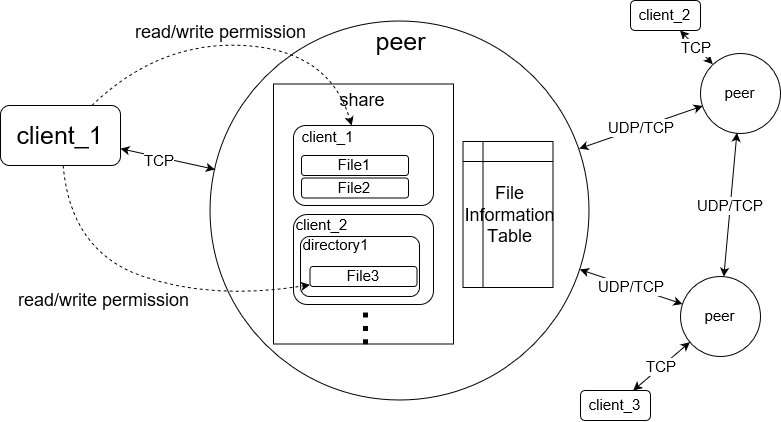
\includegraphics[width=7.8cm]{pic}
        \caption{Protocol Diagram}\label{figure}
    \end{figure}
    \section{UDP Connection}
    There are three significant aspects of our UDP implementation. We will demonstrate these characters and compare them with TCP approaches. 
    \subsection{Transfer method}
    Because of this character, we employ the datagram socket to communicate between peers. UDP is considered a connectionless protocol because it doesn't require a virtual circuit, like handshake request and response, to be established before data transfer occurs. Therefore, the UDP transmission is very fast.However, the protocol of assignment 2 is required to be the same as that of assignment 1. We designed a fake handshake protocol to fulfill this requirement. Also, we store all the successfully handshake peers in the rememberPeers list, so that we can find out all the connected peers and determine if the connected peer number exceeds the max connection number. However, the TCP approach needs a handshake process before the connection established. Besides, the connection is more reliable and stable.
    \subsection{Process data method}    
    In UDP protocol, it uses the datagram packet to receive DatagramSocket data. In each data packet, the receiver IP host and port will be saved. Thus, the data packet can be sent to the right IP address. Furthermore, the size of the datagram packets has a limitation. The max size of a datagram packet in our UDP implementation is 8196 bytes. By contrast, there is no limitation size of transmission data in the TCP protocol. Therefore, the number of transmissions is less.
    \subsection{Re-transfer data packet}    
    Since the packet size is relatively small in the UDP transmission. It is good for small file transmitting, and very fast. But, for a large file, it is going to need a lot of packets and the number of transmissions will increase as the size of a file larger. To address this issue, we employed a re-send mechanism to re-send those lost packets. While TCP protocol is more reliable because of its block control mechanism.


\end{document}